\documentclass[12pt,t]{beamer}
\usepackage{graphicx}
\usepackage[vlined]{algorithm2e}
\usepackage{times}
\usepackage{calc}
\usepackage{url}
\usepackage{soul}
\usepackage{graphicx}
\usepackage{multirow, hhline}
\usepackage{array, booktabs}
\usepackage{amsmath}
\usepackage{amssymb}
\usepackage{relsize}
\usepackage{multirow}
\usepackage{booktabs}
\usepackage{pagecolor}
\usepackage{lipsum}
\usepackage{capt-of}
\usepackage{booktabs}

\usepackage{graphicx}
\usepackage{multicol}
\usepackage[T1]{fontenc}
\usepackage{ae}
\graphicspath{{fig/}}
\setbeameroption{hide notes}
\setbeamertemplate{note page}[plain]

\usetheme{default}
\beamertemplatenavigationsymbolsempty
\hypersetup{pdfpagemode=UseNone}

\usefonttheme{professionalfonts}
\usefonttheme{serif}
\usepackage{fontspec}
\setmainfont{Karla}
\setbeamerfont{note page}{family*=pplx,size=\footnotesize} % Palatino for notes

\definecolor{foreground}{RGB}{70,70,70}
\definecolor{background}{RGB}{249, 249, 249} %24,24,24
%\definecolor{title}{RGB}{107,174,214} %107,174,214
\definecolor{title}{RGB}{70,70,70}
\definecolor{gray}{RGB}{0,0,0}
\definecolor{subtitle}{RGB}{70,70,70}
\definecolor{hilight}{RGB}{102,255,204}
\definecolor{vhilight}{RGB}{255,111,207}

\setbeamercolor{titlelike}{fg=title}
\setbeamercolor{subtitle}{fg=subtitle}
\setbeamercolor{institute}{fg=gray}
\setbeamercolor{normal text}{fg=foreground,bg=background}


\setbeamercolor{item}{fg=foreground} % color of bullets
\setbeamercolor{subitem}{fg=gray}
\setbeamercolor{itemize/enumerate subbody}{fg=gray}
\setbeamertemplate{itemize subitem}{{\textendash}}
\setbeamerfont{itemize/enumerate subbody}{size=\footnotesize}
\setbeamerfont{itemize/enumerate subitem}{size=\footnotesize}

\setbeamercolor{block title}{fg=white,bg=gray!70}
\setbeamercolor{block body}{fg=black,bg=gray!10}
\setbeamercolor{block title alerted}{fg=red,bg=gray!40}
\setbeamercolor{block title example}{fg=black,bg=green!20}
\setbeamercolor{block body example}{fg=black,bg=green!5}
\setbeamerfont{block title}{series=\bfseries}

\hypersetup{colorlinks,linkcolor=foreground,urlcolor=foreground}


\setbeamertemplate{footline}{%
    \raisebox{5pt}{\makebox[\paperwidth]{\hfill\makebox[20pt]{\color{gray}
          \scriptsize\insertframenumber}}}\hspace*{5pt}}

\addtobeamertemplate{note page}{\setlength{\parskip}{12pt}}


\newcommand{\bi}{\begin{itemize}}
\newcommand{\ei}{\end{itemize}}
\newcommand{\ig}{\includegraphics}
\newcommand{\subt}[1]{{\footnotesize \color{subtitle} {#1}}}

\let\emph\relax % there's no \RedeclareTextFontCommand
\DeclareTextFontCommand{\emph}{\bfseries\em}


\setbeamertemplate{frametitle}
{\vskip4pt
  \leavevmode
%\hbox{%
\begin{beamercolorbox}[wd=\paperwidth,ht=2ex,dp=0ex]{frametitle}%
\underline{\makebox[\paperwidth][l]{\hspace*{10pt}
\large {{\insertframetitle}}}}
\end{beamercolorbox}
%  }%
}

%\setbeamercolor{frametitle}{fg=yellow,bg=red}

\begin{document}

\AtBeginSection[]{
  \begin{frame}
  \vfill
  \centering
  \begin{beamercolorbox}[sep=8pt,center,shadow=true,rounded=true]{title}
    \underline{\makebox[0.6\paperwidth][l]{
\large {{\insertsectionhead}}}}
  \end{beamercolorbox}
  \vfill
  \end{frame}
}

\title{\large{Lecture \#14: Decision Trees for Classification}}
\subtitle{CS 109A, STAT 121A, AC 209A: Data Science}
\author{Pavlos Protopapas \and Kevin Rader}
%\institute{Harvard University}
\date{}
\titlegraphic{
   
\includegraphics[height=2cm]{iacs}
\includegraphics[height=2cm]{hogwarts}
}
{
\setbeamertemplate{footline}{} % no page number here
\frame{
  \titlepage
  
}
}


\begin{frame}{Lecture Outline}
\tableofcontents
\end{frame}

%%%%%%%%%%%%%%%%%%%%%%%%%%%%%%%%%%%%%%%%%%%%%%%%%%%%%%%%%%%%%%%%%%%%%%%%%%%%%%
\section{Motivation}

%%%%%%%%%%%%%%
\begin{frame}{Geometry of Data} 
\only<1>{
\vskip-0.4cm
Recall that \emph{logistic regression} for classification works best when the classes are well-separated in the feature space by a decision boundary defined by some equation
\[
f(x_1, \ldots, x_J) = 0 
\]
The following is a typical dataset for logistic regression with a linear boundary:
\vskip0.2cm
\begin{center}
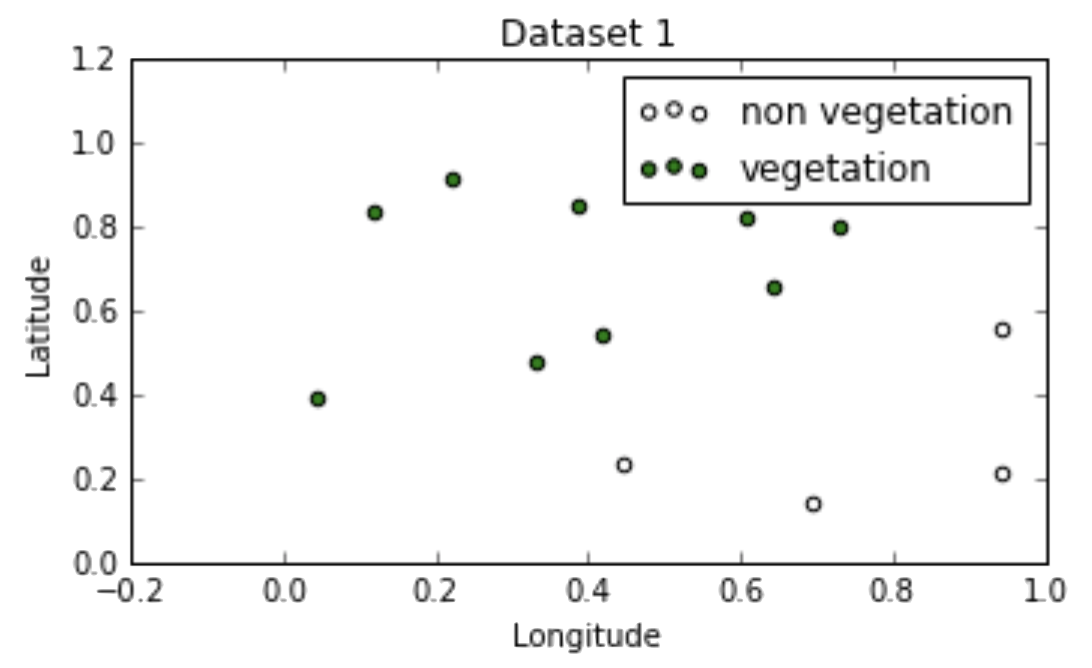
\includegraphics[width=60mm]{lecture14_g1}
\end{center}
}

\only<2-3>{
Discuss the suitability of the following datasets for logistic regression:
\vskip0.2cm
\begin{center}
\only<2>{
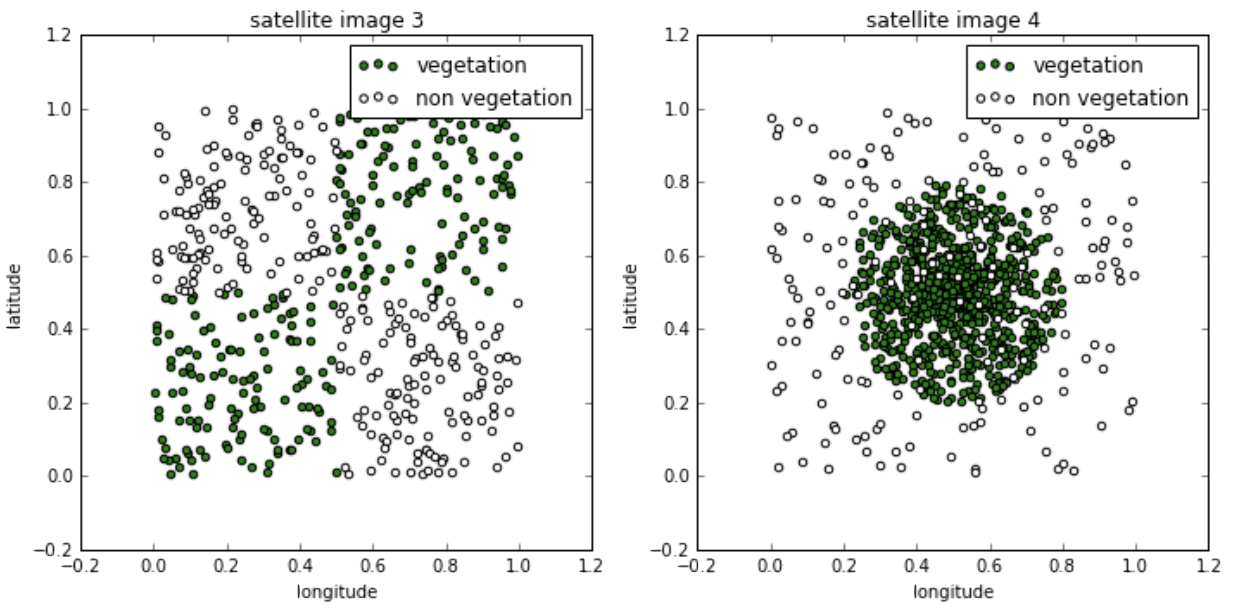
\includegraphics[width=100mm]{lecture14_g2}
}
\only<3>{
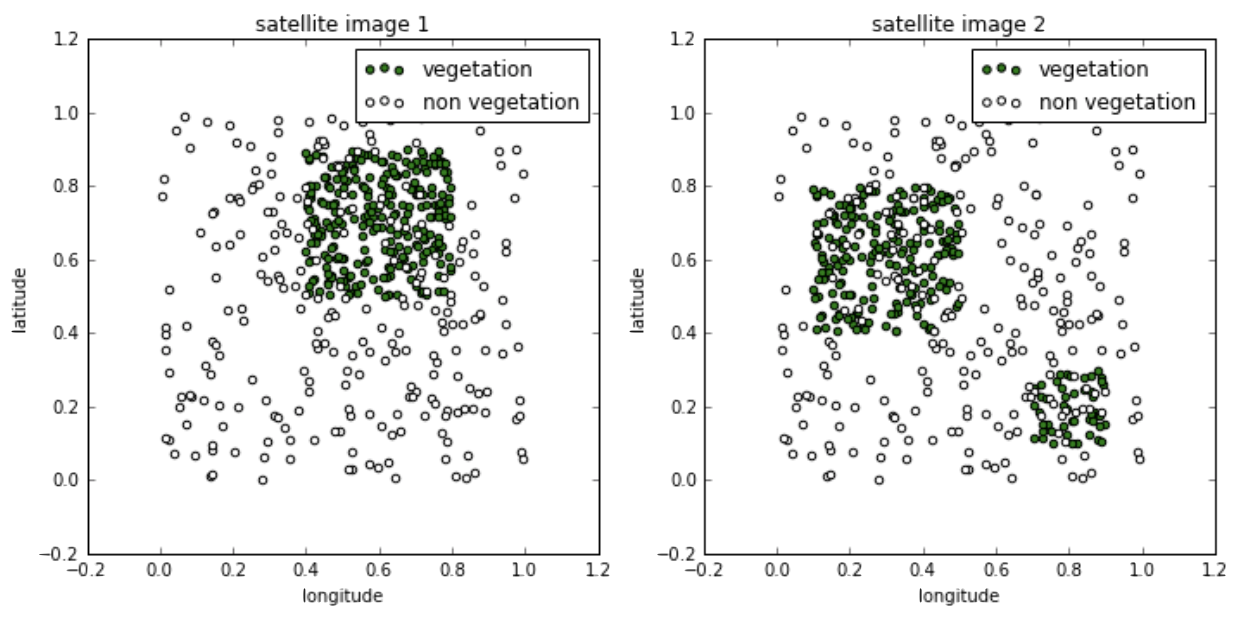
\includegraphics[width=100mm]{lecture14_g3}
}
\end{center}
}

\only<4>{
Notice that in all of the datasets the classes are still well-separated in the feature space, but \emph{the decision boundaries cannot be described by single equations}:
\vskip0.2cm
\begin{center}
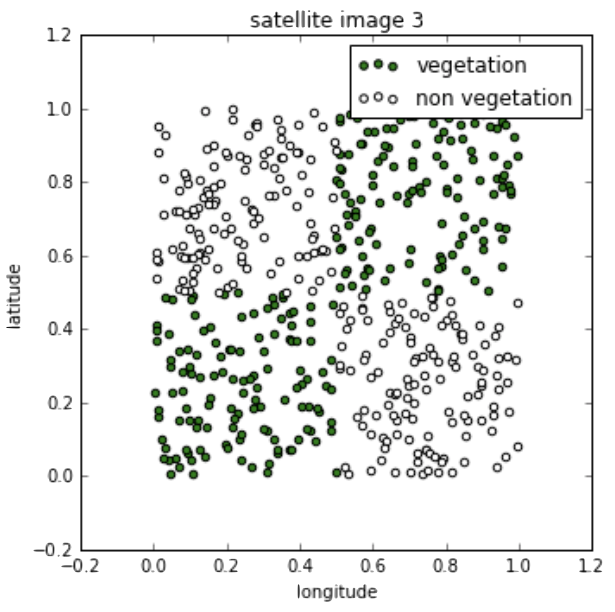
\includegraphics[width=50mm]{lecture14_g4}
\end{center}
}

\end{frame}

%%%%%%%%%%%%%%
\begin{frame}{Interpretable Models} 
\only<1>{
While logistic regression models with linear boundaries are intuitive to interpret by examining the impact of each predictor on the log-odds of a positive classification, it is less straightforward to interpret nonlinear decision boundaries in context:
\[
(x_3 + 2 x_2)^2 - x_1 + 10 = 0
\]
It would be desirable to build models with complex decision boundaries that are also easy to interpret.
}

\only<2->{
But people in every walk of life have long been using interpretable models for differentiating between classes of objects and phenomena:
\begin{center}
\only<2>{

\includegraphics[width=60mm]{lecture14_g5}
}
\only<3>{
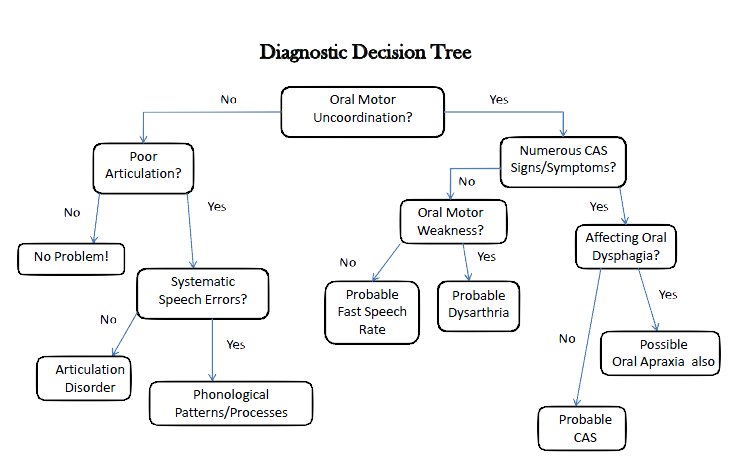
\includegraphics[width=90mm]{lecture14_g6}
}
\end{center}
}
\end{frame}

%%%%%%%%%%%%%%
\begin{frame}{Decision Trees} 
It turns out that the simple flow charts in our examples can be formulated as mathematical models for classification and these models have the properties we desire; they are:
\vskip0.2cm
\begin{enumerate}
\item interpretable by humans
\item have sufficiently complex decision boundaries
\item the decision boundaries are locally linear, each component of the decision boundary is simple to describe mathematically.
\end{enumerate}
\end{frame}

%%%%%%%%%%%%%%%%%%%%%%%%%%%%%%%%%%%%%%%%%%%%%%%%%%%%%%%%%%%%%%%%%%%%%%%%%%%%%%
\section{Decision Trees}

%%%%%%%%%%%%%%
\begin{frame}{The Geometry of Flow Charts}
\vskip-0.4cm
\only<1-2>{
Flow charts whose graph is a tree (connected and no cycles) represents a model called a \emph{decision tree}. 
\vskip0.2cm
Formally, a \emph{decision tree model} is one in which the final outcome of the model is based on a series of comparisons of the values of predictors against threshold values. 
\vskip0.2cm
\only<1>{
In a graphical representation (flow chart), 
\vskip0.2cm
\begin{itemize}
\item the internal nodes of the tree represent attribute testing
\item branching in the next level is determined by attribute value
\item leaf nodes represent class assignments
\end{itemize}
}
\only<2>{
\begin{center}
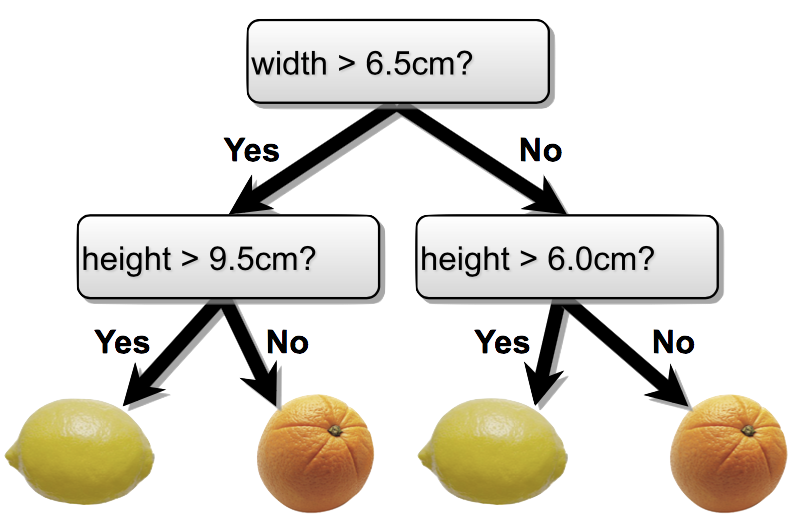
\includegraphics[width=60mm]{lecture14_g7}
\end{center}
}
}

\only<3>{
Every flow chart tree corresponds to a partition of the feature space by axis aligned lines or (hyper) planes. Conversely, every such partition can be written as a flow chart tree.
\begin{center}
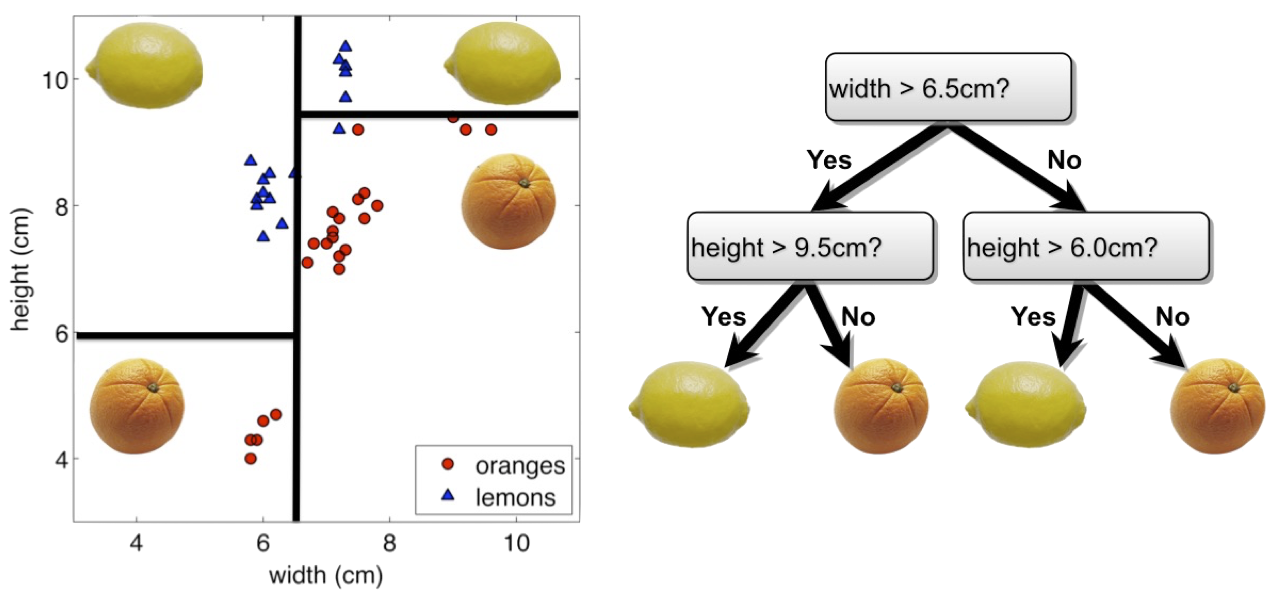
\includegraphics[width=85mm]{lecture14_g8}
\end{center} 
Each comparison and branching represents splitting a region in the feature space. Typically, at each iteration, we split once along one dimension (one predictor). 
}
\end{frame}

%%%%%%%%%%%%%%
\begin{frame}{Learning the Model} 
\only<1>{
\vskip0.4cm
Given a training set, learning a decision tree model for binary classification means to produce an `optimal' partition of the feature space with axis aligned linear boundaries, wherein each region is given a class label based on the largest class of the training points in that region.
\vskip0.2cm
}
\only<2>{
Learning the smallest `optimal' decision tree for any given set of data is NP complete for numerous simple definitions of `optimal'. Instead, we will seek a reasonably model using a greedy algorithm.
\vskip0.2cm
\begin{enumerate}
\item Start with an empty decision tree (undivided feature space)
\item Choose the `optimal' predictor on which to split and choose the `optimal' threshold value for splitting.
\item Recurse on on each new node until \emph{stopping condition} is met
\end{enumerate}
\vskip0.2cm
Now, we need only define our splitting criterion and stopping condition.
}
\end{frame}

%%%%%%%%%%%%%%
\begin{frame}{Numerical vs Categorical Attributes} 
\only<1>{
Note that the compare and branch method by which we defined regression tree works well for numerical features. 
\vskip0.2cm
However, if a feature is categorical (with more than two possible values), comparisons like $feature < threshold$ does not make sense. 
\vskip0.2cm
A simple solution is to encode the values of a categorical feature using numbers and treat this feature like a numerical variable.
\vskip0.2cm
This is indeed what some computational libraries (e.g. \texttt{sklearn}) do, however, this method has drawbacks.
}

\only<2>{
\scriptsize
\vskip-0.4cm
\begin{block}{\small Example}
Suppose the feature we want to split on is \emph{color}, and the values are: Red, Blue and Yellow. If we encode the categories numerically as:
\[
\mathrm{Red} = 0, \;\mathrm{Blue} = 1, \;\mathrm{Yellow} = 2
\]
Then the possible non-trivial splits on \emph{color} are
\begin{align*}
&\{\{ \mathrm{Red}\}, \{ \mathrm{Blue}, \mathrm{Yellow}\}\}, && \{\{ \mathrm{Red}, \mathrm{Blue}\}, \{\mathrm{Yellow}\}\}
\end{align*}
But if we encode the categories numerically as:
\[
\mathrm{Red} = 2, \;\mathrm{Blue} = 0, \;\mathrm{Yellow} = 1
\]
The possible splits are
\begin{align*}
&\{\{ \mathrm{Blue}\}, \{ \mathrm{Yellow}, \mathrm{Red}\}\}, && \{\{ \mathrm{Blue}, \mathrm{Yellow}\}, \{\mathrm{Red}\}\}
\end{align*}
\emph{Depending on the encoding, the splits we can optimize over can be different!}
\end{block}
}

\only<3>{
In practice, the effect of our choice of naive encoding of categorical variables are often negligible - models resulting from different choices of encoding will perform comparably. 
\vskip0.2cm
In cases where you might worry about encoding, there is a more sophisticated way to numerically encode the values of categorical variables so that one can optimize over all possible partitions of the values of the variable. 
\vskip0.2cm
This more principled encoding scheme is computationally more expensive but is implemented in a number of computational libraries (e.g. \texttt{R}'s \texttt{randomForest}).
}
\end{frame}



%%%%%%%%%%%%%%%%%%%%%%%%%%%%%%%%%%%%%%%%%%%%%%%%%%%%%%%%%%%%%%%%%%%%%%%%%%%%%%
\section{Splitting Criteria}

%%%%%%%%%%%%%%
\begin{frame}{Optimality of Splitting} 
While there is no `correct' way to define an optimal split, there are some common sensical guidelines for every splitting criterion:
\vskip0.2cm
\begin{itemize}
\item the regions in the feature space should grow progressively more pure with the number of splits. That is, we should see each region `specialize' towards a single class.
\vskip0.2cm
\item the fitness metric of a split should take a differentiable form (making optimization possible)
\vskip0.2cm
\item we shouldn't end up with empty regions - regions containing no training points.
\end{itemize}
\end{frame}

%%%%%%%%%%%%%%
\begin{frame}{Classification Error} 
\only<1>{
Suppose we have $J$ number of predictors and $K$ classes.  
\vskip0.2cm
Suppose we select the $j$-the predictor and split a region containing $N$ number of training points along the threshold $t_j \in \mathbb{R}$. 
\vskip0.2cm
We can assess the quality of this split by measuring the classification error made by each newly created region, $R_1, R_2$:
\[
\mathrm{Error}(i | j, t_j) = 1 - \max_k p(k | R_i)
\]
where $p(k | R_i)$ is the proportion of training points in $R_i$ that are labeled class $k$. 
}

\only<2>{
\vskip-0.4cm
\begin{block}{Example}
\begin{tabular}{c|ccl}
& Class 1& Class 2 & $\mathrm{Error}(i | j, t_j) $\\
\hline
$R_1$ & 0 & 6 & $1 - \max \{6/6, 0/6 \} = 0$\\
$R_2$ & 5 & 8 & $1 - \max \{5/13, 8/13 \} = 5/13$\\
\end{tabular}
\end{block}
We can now try to find the predictor $j$ and the threshold $t_j$ that minimizes the average classification error over the two regions, weighted by the population of the regions:
\[
\min_{j, t_j} \frac{N_1}{N} \mathrm{Error}(1 | j, t_j) + \frac{N_2}{N} \mathrm{Error}(2 | j, t_j) 
\]
where $N_i$ is the number of training points inside region $R_i$.
}
\end{frame}

%%%%%%%%%%%%%%
\begin{frame}{Gini Index} 
\only<1>{
Suppose we have $J$ number of predictors, $N$ number of training points and $K$ classes.  
\vskip0.2cm
Suppose we select the $j$-the predictor and split a region containing $N$ number of training points along the threshold $t_j \in \mathbb{R}$. 
\vskip0.2cm
We can assess the quality of this split by measuring the purity of each newly created region, $R_1, R_2$. This metric is called the \emph{Gini Index}:
\[
\mathrm{Gini}(i | j, t_j) = 1 - \sum_k p(k | R_i)^2
\]
\textbf{Question:} What is the effect of squaring the proportions of each class? What is the effect of summing the squared proportions of classes within each region? 
}

\only<2>{
\vskip-0.4cm
\begin{block}{Example}
\begin{tabular}{c|ccl}
& Class 1& Class 2 & $\mathrm{Gini}(i | j, t_j) $\\
\hline
$R_1$ & 0 & 6 & $1 -  (6/6^2 + 0/6^2)  = 0$\\
$R_2$ & 5 & 8 & $1 -  [(5/13)^2 + (8/13)^2] = 80/169$\\
\end{tabular}
\end{block}
We can now try to find the predictor $j$ and the threshold $t_j$ that minimizes the average Gini Index over the two regions, weighted by the population of the regions:
\[
\min_{j, t_j} \frac{N_1}{N} \mathrm{Gini}(1 | j, t_j) + \frac{N_2}{N}\mathrm{Gini}(2 | j, t_j) 
\]
where $N_i$ is the number of training points inside region $R_i$.
}

\end{frame}


\begin{frame}{Information Theory}
\only<1>{
\vskip-0.4cm
The last  metric for evaluating the quality of a split is motivated by metrics of uncertainty in information theory.
\vskip0.2cm
Ideally, our decision tree should split the feature space into regions such that each region represents a single class. In practice, the training points in each region is distributed over multiple classes, e.g.:
\begin{center}
\begin{tabular}{c|cc}
& Class 1& Class 2 \\
\hline
$R_1$ & 1 & 6 \\
$R_2$ & 5 & 6
\end{tabular}
\end{center}
However, though both imperfect, $R_1$ is clearly sending a stronger `signal' for a single class (Class 2) than $R_2$.
}
\only<2>{
\small
\vskip-0.4cm
One way to quantify the strength of a signal in a particular region is to analyze the distribution of classes within the region. We compute the \emph{entropy} of this distribution. 
\vskip0.2cm
For a random variable with a discrete distribution, the entropy is computed by
\[
H(X) = - \sum_{x\in X} p(x) \log_2 p(x)
\]
Higher entropy means the distribution is uniform-like (flat histogram) and thus values sampled it are `less predictable' (all possible values are equally probable). 
\vskip0.2cm
Lower entropy means the distribution has more defined peaks and valleys and thus values sampled from it are `more predictable' (values around the peaks are more probable).
}

\end{frame}


%%%%%%%%%%%%%%
\begin{frame}{Entropy} 
\only<1>{
Suppose we have $J$ number of predictors, $N$ number of training points and $K$ classes.  
\vskip0.2cm
Suppose we select the $j$-the predictor and split a region containing $N$ number of training points along the threshold $t_j \in \mathbb{R}$. 
\vskip0.2cm
We can assess the quality of this split by measuring the entropy of the class distribution in each newly created region, $R_1, R_2$:
\[
\mathrm{Entropy}(i | j, t_j) = - \sum_k p(k | R_i) \log_2 [p(k | R_i)]
\]
\textbf{Note:} we are actually computing the conditional entropy of the distribution of training points amongst the $K$ classes given that the point is in region $i$.
}

\only<2>{
\vskip-0.4cm
\begin{block}{Example}
\begin{tabular}{c|ccl}
& Class 1& Class 2 & $\mathrm{Entropy}(i | j, t_j) $\\
\hline
$R_1$ & 0 & 6 & $-  (\frac{6}{6} \log_2 \frac{6}{6} + \frac{0}{6} \log_2 \frac{0}{6} )  = 0$\\
$R_2$ & 5 & 8 & $ -  (\frac{5}{13} \log_2 \frac{5}{13}+ \frac{8}{13} \log_2 \frac{8}{13}) \approx 1.38$\\
\end{tabular}
\end{block}
We can now try to find the predictor $j$ and the threshold $t_j$ that minimizes the average entropy over the two regions, weighted by the population of the regions:
\[
\min_{j, t_j} \frac{N_1}{N} \mathrm{Entropy}(1 | j, t_j) + \frac{N_2}{N} \mathrm{Entropy}(2 | j, t_j) 
\]
}
\end{frame}

%%%%%%%%%%%%%%
\begin{frame}{Comparison of Criteria} 
\vskip-0.4cm
Recall our intuitive guidelines for splitting criteria, which of the three criteria fits our guideline the best?
\vskip0.2cm
\only<1>{
We have the following comparison of the value of the three criteria at different levels of purity (from 0 to 1) in a single region.
\begin{center}
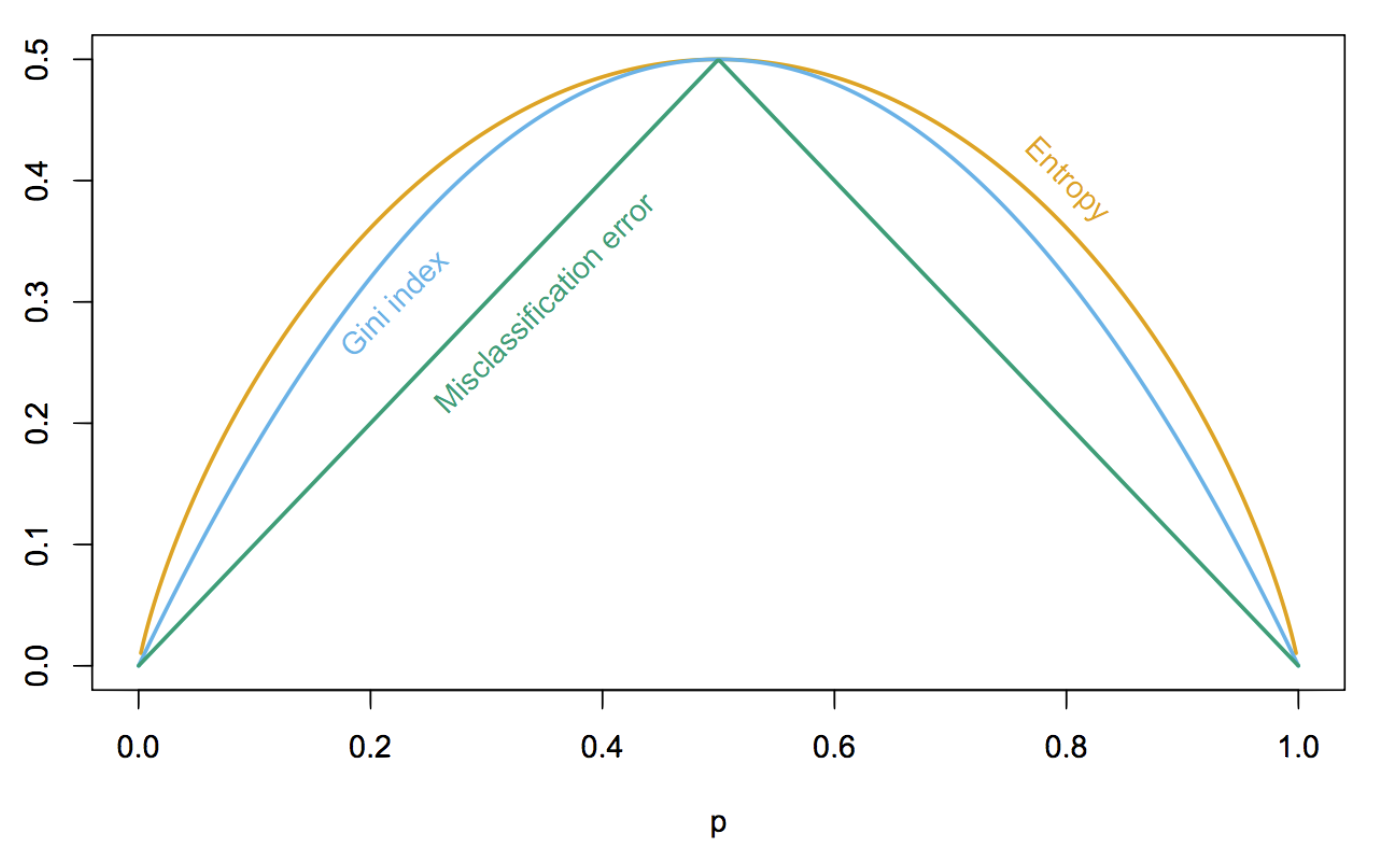
\includegraphics[width=80mm]{lecture14_g9}
\end{center}
}
\only<2>{
To note that entropy penalizes impurity the most is not to say that it is the best splitting criteria. For one, a model with purer leaf nodes on a training set may not perform better on the testing test.
\vskip0.2cm
Another factor to consider is the size of the tree (i.e. model complexity) each criteria tends to promote. 
\vskip0.2cm
To compare different decision tree models, we need to first discuss \emph{stoping conditions}.
}
\end{frame}

%%%%%%%%%%%%%%%%%%%%%%%%%%%%%%%%%%%%%%%%%%%%%%%%%%%%%%%%%%%%%%%%%%%%%%%%%%%%%%
\section{Stopping Conditions \& Pruning}

%%%%%%%%%%%%%%
\begin{frame}{Variance vs Bias} 


\only<1>{
If we don't terminate the decision tree learning algorithm manually, the tree  will continue to grow until each region defined by the model contains exact one training point (and the model attains 100\% training accuracy).
\vskip0.2cm
To prevent this from happening, we can simply stop the algorithm at a particular depth.
\vskip0.2cm
But how do we determine the appropriate depth?
}

\only<2>{
\small
\vskip-0.4cm
Consider the result of training a decision tree of various depths on a previous example dataset:
\begin{center}
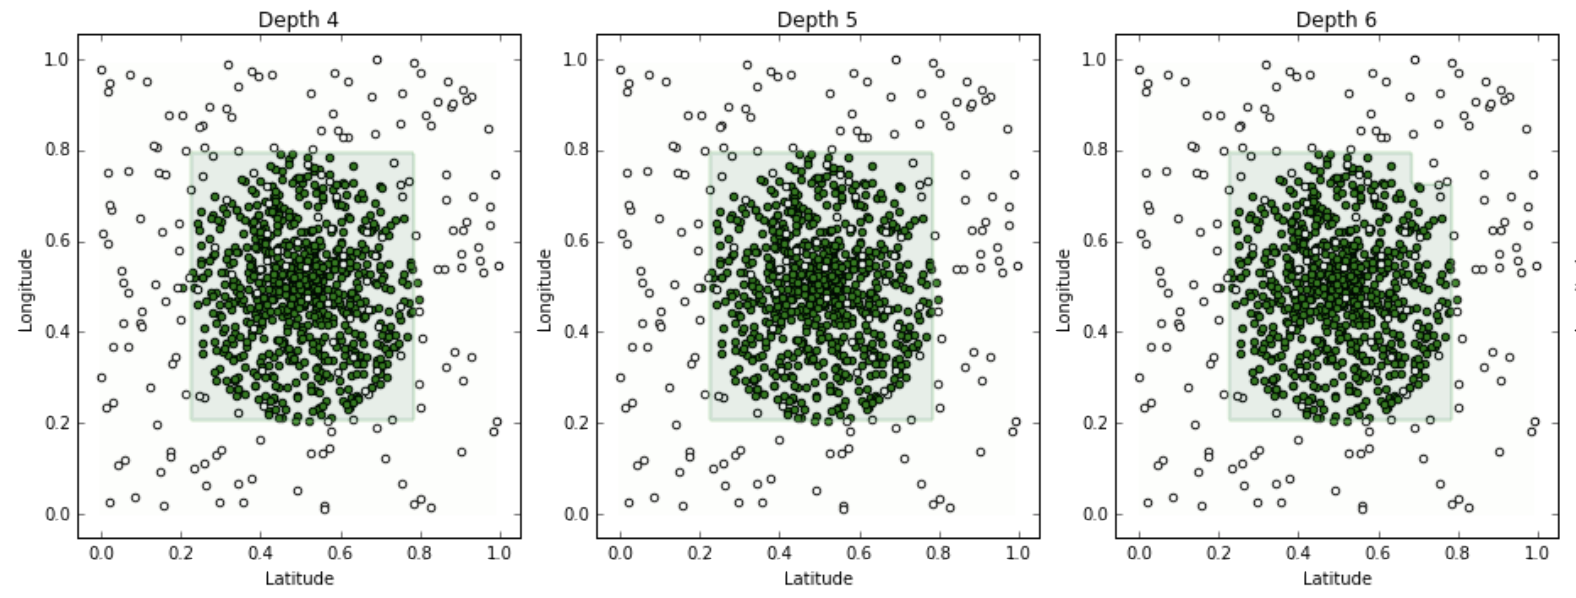
\includegraphics[width=70mm]{lecture14_g10}\\
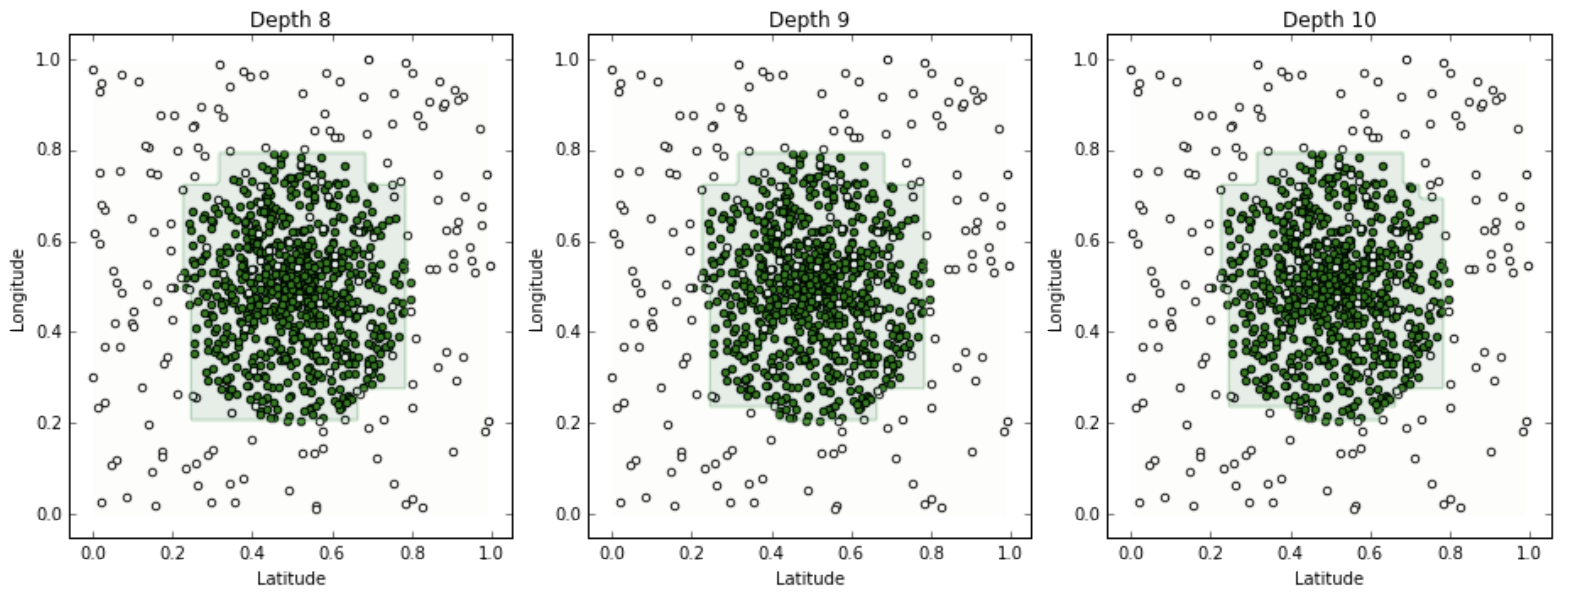
\includegraphics[width=70mm]{lecture14_g11}
\end{center}
}

\only<3>{
\vskip-0.4cm
\footnotesize
We make some observations about our models:
\begin{itemize}
\item \textbf{(Bias)} A tree of depth 4 is not a good fit for the training data - it's unable to capture the nonlinear boundary separating the two classes. 
\item \textbf{(Bias)} With an extremely high depth, we can obtain a model that correctly classifies all points on the boundary (by zig-zagging around each point). 
\item \textbf{(Variance)} The tree of depth 4 is robust to slight perturbations in the training data - the square carved out by the model is stable if you move the boundary points a bit.
\item \textbf{(Variance)} Trees of high depth are sensitive to perturbations in the training data, especially to changes in the boundary points. 
\end{itemize}
Not surprisingly, complex ones have low bias (able to capture more complex geometry in the data) but high variance (can over fit). Complex trees are also harder to interpret and more computationally expensive to train.
}

\end{frame}

%%%%%%%%%%%%%%
\begin{frame}{Stopping Conditions} 
\only<1>{
Common simple stopping conditions:
\vskip0.2cm
\begin{itemize}
\item Don't split a region if all instances in the region belong to the same class
\item Don't split a region if the number of instances in the sub-region will fall below pre-defined threshold
\item Don't split a region if the total number of leaves in the tree will exceed pre-defined threshold
\end{itemize}
\vskip0.2cm
The appropriate thresholds can be determined by evaluating the model on a held-out data set or, better yet, via cross-validation.
}
\only<2>{
More restrictive stopping conditions:
\begin{itemize}
\item Don't split a region if the class distribution of the training points inside the region are independent of the predictors
\item Compute the gain in purity, information or reduction in entropy of splitting a region $R$
\[
\text{Gain}(R) = \Delta(R) = m(R) - \frac{N_1}{N} m(R_1) -  \frac{N_2}{N} m(R_2)
\]
where $m$ is a metric like the Gini Index or entropy. Don't split if the gain is less than some pre-defined threshold.
\end{itemize}
}
\end{frame}

%%%%%%%%%%%%%%
\begin{frame}{Pruning} 

\only<1>{
Rather than preventing a complex tree from growing, we can obtain a simpler tree by `pruning' a complex one. 
\vskip0.2cm
There are many method of pruning, a common one is \emph{cost complexity pruning}, where by we select from a array of smaller subtrees of the full model that optimizes a balance of performance and efficiency.
\vskip0.2cm
That is, we measure
\[
\text{C}(T) = \text{Error}(T) + \alpha |T|
\]
where $T$ is a decision (sub) tree, $|T|$ is the number of leaves in the tree and $\alpha$ is the parameter for penalizing model complexity.
}

\only<2>{
\vskip-0.4cm
The pruning algorithm:
\begin{enumerate}
\item Start with a full tree $T_0$ (each leaf node contains exactly one training point)
\item Replace a subtree in $T_0$ with a leaf node to obtain a pruned tree $T_1$. This subtree should be selected to minimize
\[
\frac{\text{Error}(T_0) - \text{Error}(T_1)}{|T_0| - |T_1|}
\]
\item Iterate this pruning process to obtain $T_0, T_1, \ldots, T_L$, where $T_L$ is the tree containing just the root of $T_0$. 
\item Select the optimal tree $T_i$ by cross validation.
\end{enumerate}
\vskip0.2cm
\textbf{Note:} you might wonder where we are computing the cost-complexity $C(T_l)$. One can prove that this process is equivalent to explicitly optimizing $C$. 
}

\end{frame}

%%%%%%%%%%%%%%
\begin{frame}{An Example} 
[demonstrate difference between different splitting criteria]
[demonstrate difference between different stopping conditions]
[demonstrate overfitting and variance]
\end{frame}

\end{document}
